\chapter{固有时、时间膨胀与长度收缩}

我们将经常选取光速为$c=1$的单位制。在这种单位制下，一年的时间与一光年的距离可以直接比较，公式也更容易阅读。只要$c$在物理上起作用，我们就把它放回去。量纲分析足以确定它的位置。

\section{伽利略时空网格}

从爱因斯坦之前静止参考系与沿$x$轴以速度$v$运动的列车之间的关系出发：
\begin{align}
x' &= x-vt, & t'&=t.
\label{eq:l4-galilean}
\end{align}
第二个方程包含了牛顿关于普适时间的假设。即使空间原点彼此相对运动，每个观测者都使用相同的同时性切片。

假设不带撇的观测者站在轨道旁，带撇的观测者乘在列车上。列车原点满足$x'=0$，因此它在不带撇坐标中的世界线为
\begin{equation}
x=vt.
\end{equation}
这条倾斜的直线就是$t'$轴。相反，$t'=t$表明所有常$t'$的直线与常$t$的直线是相同的水平线。

\begin{figure}[H]
\centering
\includegraphics[width=0.72\textwidth]{lecture_04_figure_02.png}
\caption{伽利略变换与初始$t$-$x$网格。运动的原点将描出$x=vt$，而两个参考系保持共同的等时线。}
\lectureframe{00:03:06}
\end{figure}

对式~\eqref{eq:l4-galilean}求解不带撇的坐标，得到
\begin{align}
x&=x'+vt'=x'+vt, & t&=t'.
\end{align}
逆变换具有相同的形式，只是$v$被替换为$-v$。如果列车相对于车站向前运动，那么车站相对于列车向后运动。这种互易性在狭义相对论中仍然成立，但普适时间不再成立。

\section{洛伦兹修正}

伽利略变换无法使光速在每个惯性系中都相同。修正后的关系式，首先在$c=1$单位下为
\begin{align}
x'&=\frac{x-vt}{\sqrt{1-v^2}}, &
t'&=\frac{t-vx}{\sqrt{1-v^2}}.
\label{eq:l4-lorentz-natural}
\end{align}
恢复普通单位后得到
\begin{align}
x'&=\frac{x-vt}{\sqrt{1-v^2/c^2}}, &
t'&=\frac{t-vx/c^2}{\sqrt{1-v^2/c^2}}.
\label{eq:l4-lorentz-c}
\end{align}

\begin{figure}[H]
\centering
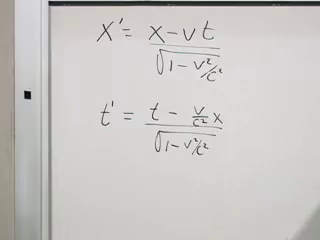
\includegraphics[width=0.74\textwidth]{lecture_04_figure_05.png}
\caption{恢复了$c$因子的洛伦兹变换。}
\lectureframe{00:09:10}
\end{figure}

对于$v\ll c$，在使用牛顿力学的场合中，$v^2/c^2$和$vx/c^2$都很小。此时式~\eqref{eq:l4-lorentz-c}约化为伽利略结果。相对论并未抛弃牛顿运动学；它确定了牛顿运动学的有效范围。

当$v=c$时，分母为零。一个惯性系不能相对于另一个惯性系以光速运动。远低于该极限时修正很小，但接近它时，$x$与$t$的混合变得不可避免。

运动是沿$x$选取的，因此横向坐标不变：
\begin{equation}
y'=y,\qquad z'=z.
\end{equation}
理解这一点的一种方法是，在列车和站台上放置相同的横向米尺。一个在两个参考系正中间运动的观测者看到两根尺以大小相等、方向相反的速度接近。这个设置没有任何特征能使一根横向尺比另一根短。

\section{沿光锥的洛伦兹变换}

有一种几何方式来解读式~\eqref{eq:l4-lorentz-natural}。将其两个方程相加：
\begin{align}
t'+x'
&=\frac{(t-vx)+(x-vt)}{\sqrt{1-v^2}}\\
&=(t+x)\frac{1-v}{\sqrt{1-v^2}}\\
&=(t+x)\sqrt{\frac{1-v}{1+v}}.
\label{eq:l4-null-plus}
\end{align}
以互补的顺序相减：
\begin{align}
t'-x'
&=\frac{(t-vx)-(x-vt)}{\sqrt{1-v^2}}\\
&=(t-x)\frac{1+v}{\sqrt{1-v^2}}\\
&=(t-x)\sqrt{\frac{1+v}{1-v}}.
\label{eq:l4-null-minus}
\end{align}

\begin{figure}[H]
\centering
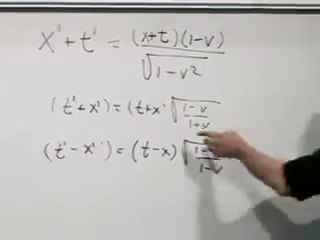
\includegraphics[width=0.75\textwidth]{lecture_04_figure_06.png}
\caption{用零组合$t+x$和$t-x$重写的洛伦兹变换。它们的比例因子互为倒数。}
\lectureframe{00:18:45}
\end{figure}

组合$t+x$和$t-x$是沿两个$45^\circ$类光方向的坐标。一个推进会压缩其中一个方向，并以倒数因子拉伸另一个方向。它不会使其中任何一个方向偏离$45^\circ$。因此光线仍然是光线，这就是光速不变性的时空图景。

\begin{classroomqa}
\audiencequestion{正中间的观测者看到一个对称的实验，但这如何为列车和站台上的观测者确立结果？\lecturetimestamp{00:20:48}}
\lecturerresponse{这里还使用了另一个事实：事件的重合是不变的。如果两根尺的端点相遇，那次相遇就是一个时空事件。每个惯性观测者可以给它赋予不同的坐标，但没有人能把一次重合分成两个不同的位置。在相应端点相遇处发出的闪光使这些事件在操作上可被探测。正中间参考系的对称性以及两个端点重合的不变性，确立了横向长度一致。}
\end{classroomqa}

\begin{classroomqa}
\audiencequestion{代表中间参考系的骑自行车者是否必须物理上位于两根杆的中点？\lecturetimestamp{00:22:25}}
\lecturerresponse{不。参考系是一整套由观察者和时钟构成的网络，而不是位于某一位置的一只眼睛。骑自行车者可以在稍后接收到端点发出的闪光，并推断它们源自何处。重要的是每个发射事件在时空中的位置，而不是光最终在哪里被接收到。}
\end{classroomqa}

相继速度的合成是同一变换的另一个推论，但有意留到下一讲。当前的任务是确定运动时钟所测量的不变量。

\section{不变间隔}

对于普通笛卡尔坐标轴的旋转，量$x^2+y^2$保持不变。洛伦兹变换保持的是另一个二次型。由式~\eqref{eq:l4-lorentz-natural}，
\begin{align}
t'^2-x'^2
&=\frac{(t-vx)^2-(x-vt)^2}{1-v^2}\\
&=\frac{t^2-2vtx+v^2x^2-x^2+2vtx-v^2t^2}{1-v^2}\\
&=t^2-x^2.
\label{eq:l4-interval}
\end{align}
交叉项相消，剩余的分子含有公因子$1-v^2$。

\begin{figure}[H]
\centering
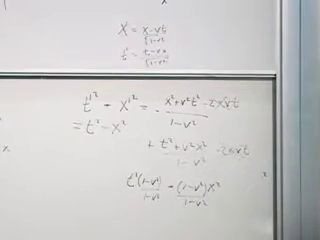
\includegraphics[width=0.76\textwidth]{lecture_04_figure_07.png}
\caption{黑板上对$t'^2-x'^2=t^2-x^2$的推导。}
\lectureframe{00:33:15}
\end{figure}

在三维空间中，不变量为
\begin{equation}
t'^2-x'^2-y'^2-z'^2=t^2-x^2-y^2-z^2
\end{equation}
以$c=1$为单位。更一般地，对于两个事件，我们使用坐标差：
\begin{equation}
\Delta s^2
=c^2\Delta t^2-\Delta x^2-\Delta y^2-\Delta z^2.
\label{eq:l4-spacetime-interval}
\end{equation}
每个惯性观察者都同意这个数，尽管他们对其中的时间项和空间项分别并不一致。

\section{固有时与运动时钟}

想象一个由静止观察者组成的格点，他们的时钟已通过交换光信号同步。他们的读数定义了坐标时间$t$。现在让一只手表穿过这个格点。它自身的读数沿着其世界线跟随这只手表；该读数就是固有时。

对于两个类时分离的事件，定义
\begin{equation}
c^2\Delta\tau^2
=c^2\Delta t^2-\Delta x^2-\Delta y^2-\Delta z^2.
\label{eq:l4-proper-time}
\end{equation}
在一维空间中，当$c=1$时，这简单地就是
\begin{equation}
\Delta\tau=\sqrt{\Delta t^2-\Delta x^2}.
\end{equation}
平方根与普通距离的公式类似，但负号改变了几何。

有三种情况：
\begin{align}
\Delta t^2-\Delta x^2 &>0 &&\text{timelike},\\
\Delta t^2-\Delta x^2 &=0 &&\text{lightlike},\\
\Delta t^2-\Delta x^2 &<0 &&\text{spacelike}.
\end{align}
在光锥内部，固有时为实数。在光锥上，即$x=\pm t$处，即使事件不必重合，固有时也为零。光线恰好可以连接这样的事件。在光锥外部，间隔是类空的；用实固有距离$\sqrt{\Delta x^2-\Delta t^2}$来描述它比用虚时钟时间更好。

\begin{figure}[H]
\centering
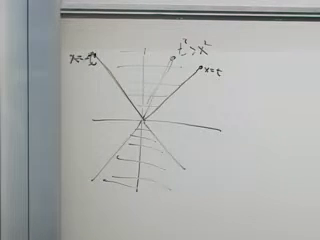
\includegraphics[width=0.73\textwidth]{lecture_04_figure_08.png}

\vspace{0.8em}

\begin{tikzpicture}[x=1.0cm,y=1.0cm]
\draw[->] (-3.3,0) -- (3.3,0) node[right] {$x$};
\draw[->] (0,-0.4) -- (0,4.0) node[above] {$t$};
\draw[thick] (0,0) -- (3.0,3.0) node[above right] {$x=t$};
\draw[thick] (0,0) -- (-3.0,3.0) node[above left] {$x=-t$};
\node at (0,2.0) {timelike};
\node at (2.25,1.05) {spacelike};
\node at (-2.25,1.05) {spacelike};
\end{tikzpicture}
\caption{黑板上的光锥以及对类时、类光、类空间隔的清晰分类。}
\lectureframe{00:38:40}
\end{figure}

为什么式~\eqref{eq:l4-proper-time}等于时钟读数？对于静止的时钟，$\Delta x=0$，所以$\Delta\tau=\Delta t$。对于匀速运动的时钟，选择该时钟在其中静止的带撇参考系。在那里$\Delta x'=0$，而不变性给出
\begin{equation}
\Delta\tau
=\sqrt{\Delta t'^2-\Delta x'^2}
=\Delta t'.
\end{equation}
因此运动时钟记录的就是固有时。

\begin{classroomqa}
\audiencequestion{``事件之间的间隔''和``时钟的读数''是否被用作同一事物的两个名称？
\lecturetimestamp{00:44:49}}
\lecturerresponse{当一个理想时钟从一个事件惯性运动到另一个事件时，它们重合。不变间隔是一个几何量；共动时钟的端点读数之差是它的物理测量。静止的坐标时钟通常记录不同的坐标时间间隔。}
\end{classroomqa}

\section{时间膨胀与同时性}

考虑运动参考系的原点。它的世界线满足
\begin{equation}
x'=0,\qquad x=vt.
\end{equation}
同一条斜线既是运动时钟的路径，也是$t'$轴。

\begin{figure}[H]
\centering
\includegraphics[width=0.72\textwidth]{lecture_04_figure_03.png}
\caption{运动原点：$x=vt$、$x'=0$和$t'$轴是同一条世界线的三种描述。}
\lectureframe{00:48:18}
\end{figure}

对共同原点和该世界线上稍后一点应用不变间隔：
\begin{align}
t'^2-x'^2&=t^2-x^2,\\
t'^2&=t^2-v^2t^2,\\
t'&=t\sqrt{1-v^2}.
\label{eq:l4-time-dilation-natural}
\end{align}
恢复$c$后，
\begin{equation}
\Delta\tau=\Delta t\sqrt{1-\frac{v^2}{c^2}}
=\frac{\Delta t}{\gamma},
\qquad
\gamma=\frac{1}{\sqrt{1-v^2/c^2}}.
\label{eq:l4-time-dilation}
\end{equation}

\begin{figure}[H]
\centering
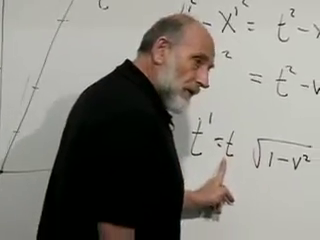
\includegraphics[width=0.73\textwidth]{lecture_04_figure_09.png}
\caption{黑板上的时间膨胀结果：运动时钟累积$t'=t\sqrt{1-v^2}$，单位取$c=1$。}
\lectureframe{00:50:45}
\end{figure}

静止观察者说运动时钟走得慢。互易性要求运动观察者对静止时钟说同样的话。这并不矛盾，因为两种描述比较的是不同的远距事件对。

确实，式~\eqref{eq:l4-lorentz-natural}中$t'$取常数值满足
\begin{equation}
t-vx=\text{constant}.
\label{eq:l4-simultaneity}
\end{equation}
运动观察者的同时线相对于水平线$t=\text{constant}$是倾斜的。每个观察者把不同的一组远距时钟读数称为同时的。一旦保持这种差异可见，时钟的相互变慢就是一致的。

\begin{figure}[H]
\centering
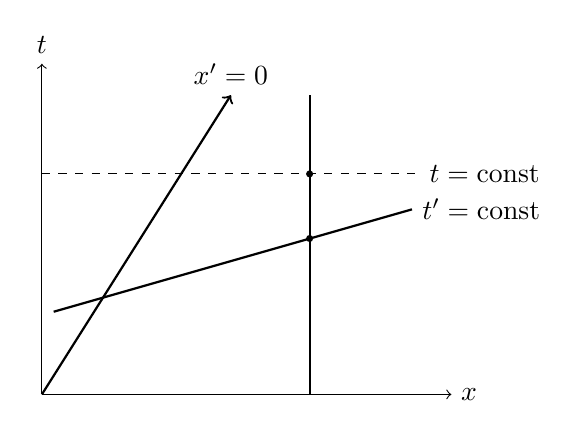
\begin{tikzpicture}[x=1cm,y=1cm]
\draw[->] (0,0) -- (0,4.2) node[above] {$t$};
\draw[->] (0,0) -- (5.2,0) node[right] {$x$};
\draw[thick,->] (0,0) -- (2.4,3.8) node[above] {$x'=0$};
\draw[dashed] (0,2.8) -- (4.8,2.8)
  node[right] {$t=\mathrm{const}$};
\draw[thick] (0.15,1.05) -- (4.7,2.35)
  node[right] {$t'=\mathrm{const}$};
\draw[thick] (3.4,0) -- (3.4,3.8);
\fill (3.4,2.8) circle (0.045);
\fill (3.4,1.98) circle (0.045);
\end{tikzpicture}
\caption{互易时间膨胀比较的是不同同时切片上的时钟读数。}
\end{figure}

\section{孪生路径}

两个双胞胎从同一事件出发。一个留在$x=0$处。另一个以速度$v$向外运动，然后反向并以相同速度返回。当他们重逢时，他们比较每一个可以作为时钟的物理过程：手表、心跳、新陈代谢或衰老本身。

设每一半旅程在家的参考系中花费坐标时间$T$。留在家中的双胞胎的固有时为
\begin{equation}
\tau_{\mathrm{home}}=2T.
\end{equation}
转向事件具有坐标$(vT,T)$。因此第一段旅行贡献
\begin{align}
\tau_{\mathrm{leg}}
&=\sqrt{T^2-v^2T^2}
=T\sqrt{1-v^2}.
\end{align}
返回段贡献相同的量，因此
\begin{equation}
\tau_{\mathrm{travel}}=2T\sqrt{1-v^2}<2T.
\label{eq:l4-twin}
\end{equation}

\begin{figure}[H]
\centering
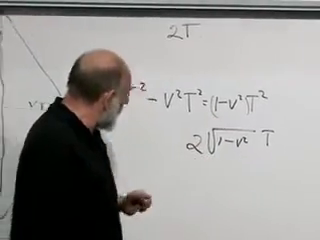
\includegraphics[width=0.73\textwidth]{lecture_04_figure_10.png}

\vspace{0.8em}

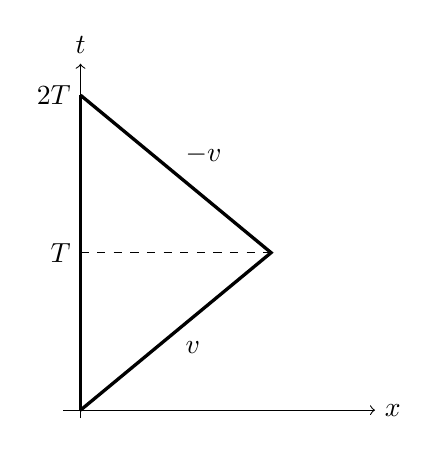
\begin{tikzpicture}[x=1.1cm,y=1cm]
\draw[->] (-0.2,0) -- (3.4,0) node[right] {$x$};
\draw[->] (0,-0.1) -- (0,4.4) node[above] {$t$};
\draw[very thick] (0,0) -- (0,4);
\draw[very thick] (0,0) -- (2.2,2) -- (0,4);
\draw[dashed] (0,2) -- (2.2,2);
\node[left] at (0,2) {$T$};
\node[left] at (0,4) {$2T$};
\node[below right] at (1.1,1.0) {$v$};
\node[above right] at (1.1,3.0) {$-v$};
\end{tikzpicture}
\caption{留在家中的世界线和两段旅行。它们的固有时不同，因为它们是时空中的不同路径。}
\lectureframe{00:59:35}
\end{figure}

年龄不等并不矛盾。旅行路径包含一个转向，并且与直线在家的路径之间不存在单一惯性系对称性的关系。在普通欧几里得几何中，两点之间的直线路线和折线路线也有不同的长度。闵可夫斯基几何反转了哪条路径具有更大间隔，但比较仍然是几何的。

\section{加速度与理想时钟}

\begin{classroomqa}
\audiencequestion{在转向处物理情况不同，旅行者加速。这是否使时钟计算失效？
\lecturetimestamp{01:02:19}}
\lecturerresponse{加速度是真实的，并有助于识别不对称性；不应将其辩解掉。尖锐的拐角只是理想化的画法，可以圆滑化为有限的转向。进一步的物理假设是，一个足够小、构造良好的时钟对适度的加速度不敏感，并继续记录固有时。一个大或脆弱的时钟可能变形或损坏，但那是机制的缺陷，而不是时空间隔的缺陷。}
\end{classroomqa}

这个理想时钟假设并非仅从洛伦兹变换推导出来。它通过实际时钟机制的行为来检验。原子比横跨数百英里的时钟要好得多的近似，因为紧凑的机制在加速度或引力下更难变形。仅仅援引广义相对论的名字并不能消除这个物理问题；人们仍然必须知道所选机制如何响应其环境。

\begin{classroomqa}
\audiencequestion{能否将加速轨迹分解为短间隔，使得惯性分析在这些间隔上仍然有效？\lecturetimestamp{01:09:08}}
\lecturerresponse{可以。将曲线分成短的、近似直线的段，计算每一段上的固有时，然后将结果相加。这是用许多小线段求普通曲线长度的时空类比。在连续极限下，
\[
\tau=\int \sqrt{1-\frac{v(t)^2}{c^2}}\,dt,
\]
对于在惯性坐标系中描述的平直时空中的运动。}
\end{classroomqa}

\section{双胞胎看到什么}

最终的时钟读数可以通过发送光脉冲来操作化。在两条世界线上标记一秒的固有时间隔，并让每个双胞胎在每个标记处发出一个脉冲。在外出段，从另一个双胞胎接收到的脉冲被拉开。在返回段，它们成束到达。这是直接在时空图上表达的爱因斯坦相对论多普勒效应。

\begin{figure}[H]
\centering
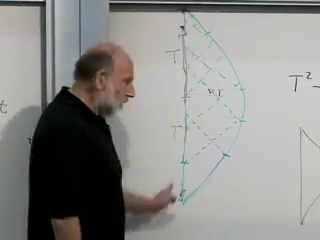
\includegraphics[width=0.73\textwidth]{lecture_04_figure_11.png}
\caption{在家和旅行世界线之间交换的光信号。外出段稀疏的到达和返回段压缩的到达解释了每一个发出的脉冲。}
\lectureframe{01:12:55}
\end{figure}

故事中没有参考系消失。每个观察者最终都会接收到对方发出的所有脉冲，但它们的接收率取决于相对运动。对于两条路径，外出的红移和返回的蓝移不是等持续时间效应，因此计数所有接收到的脉冲与固有时比较一致。

\begin{classroomqa}
\audiencequestion{如果返回的旅行者接收到蓝移的光，旅行者能否收集到比光源发出的更多的能量？
\lecturetimestamp{01:13:50}}
\lecturerresponse{这个问题需要能量的相对论定义和参考系依赖性，而这些尚未展开。这是合理的，但仅凭坐标和脉冲计数不足以解决能量记账，尤其是对于加速观察者。因此答案应推迟，而不是猜测。}
\end{classroomqa}

\section{一个闭合的空间方向}

\begin{classroomqa}
\audiencequestion{假设有一个空间方向是紧致的。一个孪生子能否沿它匀速运动，回到出发点，并且完全避免加速？那么又是什么区分了这对孪生子？\lecturetimestamp{01:15:14}}
\lecturerresponse{空间应当被内在地想象为一个圆柱面，而不是一张弯曲嵌入更大空间中的薄片；这里不必存在径向加速度。然而，返回的观测者会遇到这样一个整体事实：相同的地点会重复出现。这表明存在一种不对称性，但要给出完整答案，需要对带有空间认同的狭义相对论作细致处理。这个问题在此留作开放，而不是即兴作答。}
\end{classroomqa}

\begin{figure}[H]
\centering
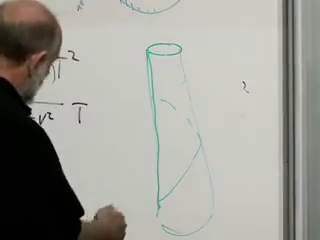
\includegraphics[width=0.72\textwidth]{lecture_04_figure_04.png}

\vspace{0.8em}

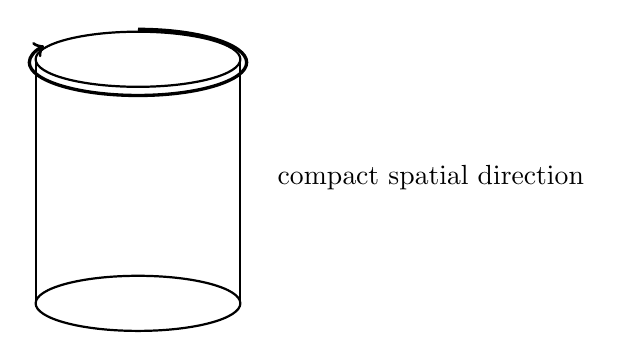
\begin{tikzpicture}[x=1cm,y=1cm]
\draw[thick] (0,0) ellipse (1.3 and 0.35);
\draw[thick] (-1.3,0) -- (-1.3,-3.1);
\draw[thick] (1.3,0) -- (1.3,-3.1);
\draw[thick] (0,-3.1) ellipse (1.3 and 0.35);
\draw[->,very thick] (0.0,0.38) arc (90:-210:1.38 and 0.42);
\node[right] at (1.65,-1.5) {compact spatial direction};
\end{tikzpicture}
\caption{黑板上所画的紧致空间问题，配有一个干净的内禀圆柱面。这是一个关于整体认同的问题，而不是关于绕着一个嵌入额外径向维度的圆柱面运动的问题。}
\lectureframe{01:17:56}
\end{figure}

\section{长度是在同时性切片上测量的}

对于狭义相对论问题，首先要画出时空图。取一根在未加撇系中静止的米尺，其端点位于$x=0$和$x=1$。随着时间流逝，两个端点描出竖直的世界线。这根尺在它们之间扫出一条带状区域。

运动的观测者必须在运动时间$t'$的同一个值上测量两个端点。由式~\eqref{eq:l4-simultaneity}，过原点且满足$t'=0$的切片在$c=1$单位下满足
\begin{equation}
t=vx
\end{equation}
它与右端点$x=1$相交于$t=v$。

\begin{figure}[H]
\centering
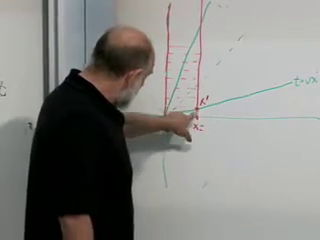
\includegraphics[width=0.73\textwidth]{lecture_04_figure_12.png}

\vspace{0.8em}

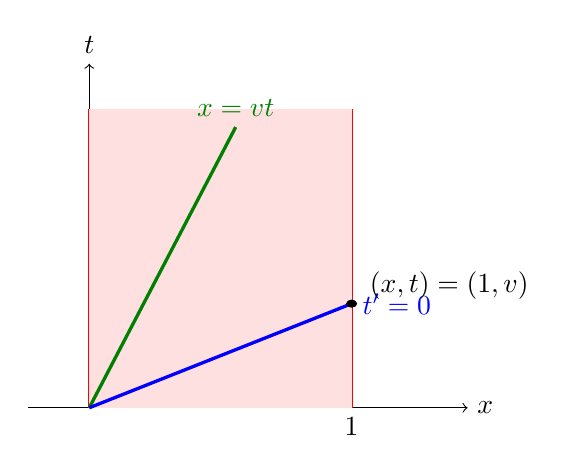
\begin{tikzpicture}[x=1.55cm,y=1.15cm]
\draw[->] (-0.5,0) -- (3.1,0) node[right] {$x$};
\draw[->] (0,0) -- (0,3.8) node[above] {$t$};
\draw[very thick,red] (0,0) -- (0,3.3);
\draw[very thick,red] (2.15,0) -- (2.15,3.3);
\fill[red!12] (0,0) rectangle (2.15,3.3);
\draw[very thick,green!50!black] (0,0) -- (1.2,3.1)
  node[above] {$x=vt$};
\draw[very thick,blue] (0,0) -- (2.15,1.15)
  node[right] {$t'=0$};
\fill (2.15,1.15) circle (0.045);
\node[right] at (2.22,1.35) {$(x,t)=(1,v)$};
\node[below] at (2.15,0) {$1$};
\end{tikzpicture}
\caption{一根静止的杆扫出一条时空带状区域。运动观测者所测的长度，是其端点在一个$t'=\mathrm{const}$切片上的间隔。}
\lectureframe{01:24:20}
\end{figure}

所选端点间隔是类空的，因此使用不变量的正空间形式：
\begin{equation}
x'^2-t'^2=x^2-t^2.
\end{equation}
在所选端点处，$t'=0$，$x=1$，且$t=v$。因此
\begin{align}
x'^2&=1-v^2,\\
x'&=\sqrt{1-v^2}.
\end{align}
于是，静长度$L$在运动系中被测得为
\begin{equation}
L'=L\sqrt{1-v^2/c^2}=\frac{L}{\gamma}.
\label{eq:l4-length-contraction}
\end{equation}

\begin{figure}[H]
\centering
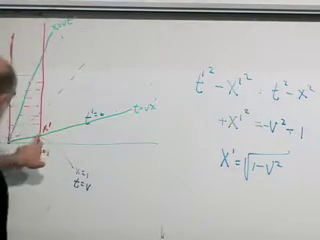
\includegraphics[width=0.76\textwidth]{lecture_04_figure_13.png}
\caption{完整的长度收缩作图以及单位静长度对应的黑板结果$x'=\sqrt{1-v^2}$。}
\lectureframe{01:28:10}
\end{figure}

相反的陈述同样成立：站台观测者赋予列车纵向米尺的长度更短。两位观测者又一次选择了不同的同时端点事件，因此这种互易性并不矛盾。

\section{结尾的问题}

\begin{classroomqa}
\audiencequestion{除了光之外，还有什么以光速传播？特别是引力呢？\lecturetimestamp{01:29:29}}
\lecturerresponse{广义相对论预言引力波以$c$传播。在这次讲座之时，证据间接来自双脉冲星等系统；引力波尚未被直接探测到。\editorialnote{在这次2006讲座之后，实验状况发生了变化。LIGO于2015年直接探测到GW150914，而对GW170817及其电磁对应体的联合观测于2017年表明，引力与光的传播速度在$10^{15}$分之几的精度内一致。参见\url{https://ligo.org/detections/gw150914/}和
\url{https://doi.org/10.1103/PhysRevLett.119.251302}。}}
\end{classroomqa}

\begin{classroomqa}
\audiencequestion{一名宇航员能否在比以光年表示的该距离更短的固有时内穿越许多光年的距离？那是否意味着运动得比光还快？\lecturetimestamp{01:30:38}}
\lecturerresponse{宇航员的固有时为
$\sqrt{\Delta t^2-\Delta x^2}$，它小于坐标时$\Delta t$。在宇航员的惯性系中，恒星之间的距离发生了洛伦兹收缩。恒星以速度$-v$运动，并不比光快；只是需要穿越的收缩后距离更短。}
\end{classroomqa}

如果宇航员从静止开始并加速，那么描述会在一系列瞬时惯性系之间发生变化。在此期间，赋予恒星的距离可以改变。人们不能对整个加速历史施加一个固定的洛伦兹变换，但总固有时仍可通过沿世界线累加各贡献而得到。同样的陈述也适用于一个真实的孪生子：他发射、转向并减速，而不是以巡航速度出生。

\begin{classroomqa}
\audiencequestion{这些困惑是否源于把时间当作特殊的存在？我们是否必须称它为第四维？\lecturetimestamp{01:36:43}}
\lecturerresponse{不必从“时间是第四维”这一口号出发。洛伦兹变换本身就迫使空间与时间相互混合，而间隔$t^2-x^2-y^2-z^2$则将它们视为同一几何的组成部分，只是时间与空间带有不同的符号。在低速下，这种混合变得可以忽略，熟悉的牛顿直觉重新出现。然而在相对论速度下，空间与时间不能被视为从根本上彼此脱耦。}
\end{classroomqa}

因此，时间膨胀、长度收缩、双生子比较以及缩短的旅行时间并非各自独立的把戏。它们都源自三个习惯：确定被比较的事件，画出它们的时空几何，并利用不变间隔。